% Original editable schematic derived from main.tex preprocessing/model methods.
% No measured waveform, participant data, or predicted probabilities are depicted.
% TikZ source prepared with OpenAI Codex assistance; no image-generation model used.
\documentclass[tikz,border=5pt]{standalone}
\usepackage[T1]{fontenc}
\usepackage{newtxtext,newtxmath}
\usetikzlibrary{arrows.meta,positioning}
\definecolor{ink}{HTML}{193C58}
\definecolor{bluefill}{HTML}{EDF4FA}
\definecolor{greenfill}{HTML}{EFF7F2}
\begin{document}
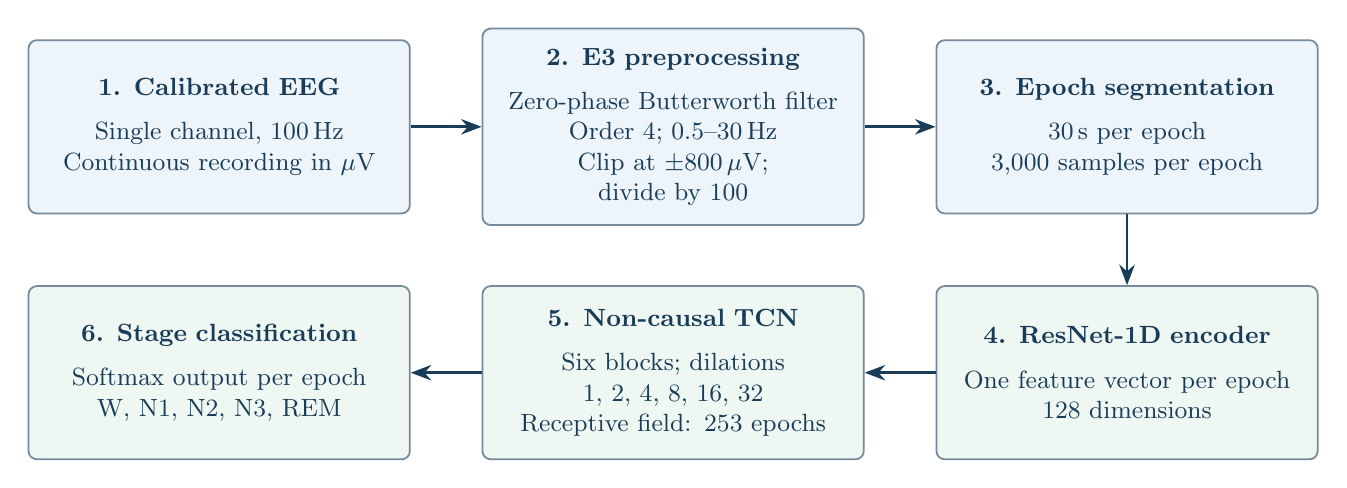
\begin{tikzpicture}[
  font=\small,text=ink,
  box/.style={draw=ink!60,rounded corners=3pt,line width=.65pt,
    fill=bluefill,text width=4.35cm,minimum height=2.2cm,align=center,inner sep=7pt},
  flow/.style={-{Stealth[length=2.6mm]},line width=1pt,draw=ink},
  node distance=9mm and 9mm]
\node[box] (input) {\textbf{1. Calibrated EEG}\\[5pt]
  Single channel, 100\,Hz\\Continuous recording in $\mu$V};
\node[box,right=of input] (prep) {\textbf{2. E3 preprocessing}\\[5pt]
  Zero-phase Butterworth filter\\Order 4; 0.5--30\,Hz\\
  Clip at $\pm800\,\mu$V; divide by 100};
\node[box,right=of prep] (epoch) {\textbf{3. Epoch segmentation}\\[5pt]
  30\,s per epoch\\3,000 samples per epoch};
\node[box,fill=greenfill,below=of epoch] (encoder) {\textbf{4. ResNet-1D encoder}\\[5pt]
  One feature vector per epoch\\128 dimensions};
\node[box,fill=greenfill,left=of encoder] (tcn) {\textbf{5. Non-causal TCN}\\[5pt]
  Six blocks; dilations 1, 2, 4, 8, 16, 32\\Receptive field: 253 epochs};
\node[box,fill=greenfill,left=of tcn] (output) {\textbf{6. Stage classification}\\[5pt]
  Softmax output per epoch\\W, N1, N2, N3, REM};
\draw[flow] (input) -- (prep);
\draw[flow] (prep) -- (epoch);
\draw[flow] (epoch) -- (encoder);
\draw[flow] (encoder) -- (tcn);
\draw[flow] (tcn) -- (output);
\end{tikzpicture}
\end{document}
